\documentclass[a4paper]{article}

\usepackage[utf8]{inputenc}
\usepackage{mathtools,amssymb,amsthm}
\usepackage{geometry}
\geometry{
	a4paper,
	top=28mm,
	bottom=28mm,
	left=24mm,
	right=24mm
}
\usepackage{fancyhdr} % Kopfzeile
\usepackage{accents}
\usepackage{enumitem}
\usepackage{framed}
\usepackage{ulem}
\usepackage{adjustbox} % Used to constrain images to a maximum size 
\usepackage{float}

% benutzerdefinierte Kommandos
\newcommand{\crown}[1]{\overset{\symking}{#1}}
\newcommand{\xcrown}[1]{\accentset{\symking}{#1}}

\makeatletter
\newcommand*{\rom}[1]{\expandafter\@slowromancap\romannumeral #1@}
\makeatother
%
\theoremstyle{plain}
\newtheorem{lemma}{Lemma}
\newtheorem*{satz}{Satz}
\newtheorem*{zz}{Zu zeigen}
\newtheorem*{formel}{Formel}



% Kopfzeile
\pagestyle{fancy}
\fancyhf{}
\rhead{405592 Victor, 405661 Pantelis, 395220 Duc}
\lhead{\textbf{Mathematical Physics I}, Jan Techter (Mon 10-12)}
\cfoot{Page \thepage}

\setlength\parindent{0pt}


\begin{document}
\section*{Exercise 10.1}
\begin{enumerate}[label=(\alph*)]
	\item The potential energy is defined as $U(q) = \frac{\alpha}{q} + \ln(\frac{q^2}{1+q^2})$ where $q \in \mathbb R$. The force acting on a particle at position $q$ is given by $F(q) = - \frac{d}{dq}U.$ Thus to get the force field, we derive $U$.
	\begin{align*}
		U'(q) = \frac{\alpha}{q^2} + \frac{1+q^2}{q^2} \cdot \frac{2q(1+q^2) - 2q^3}{q^2(1+q^2)^2} = -\frac{\alpha}{q^2} + \frac{(1+q^2)2q}{q^2(1+q^2)^2} &= \frac{-\alpha(1+q^2)^2 + 2q(1+q^2)}{q^2(1+q^2)^2} \\
		&= \frac{-\alpha(1+q^2) + 2q}{q^2(1+q^2)} \\
		&= -\frac{\alpha q^2 + \alpha - 2q}{q^2(1+q^2)}.
	\end{align*}
	So we get that 
	\[
		F(q) = -U'(q) = \frac{  \alpha q^2 + \alpha - 2q}{q^2(1+q^2)}.
	\]
	Newtons second law states $F(q) = m \ddot q $ and due to $m=1$ we obtain
	\[
		\ddot q = \frac{  \alpha q^2 + \alpha - 2q}{q^2(1+q^2)} \tag{\text{Newton's equation}}.
	\]
	The first order system of differential equations is
	\begin{align*}
		\begin{cases}
			\dot q = v \\
			\dot v = \frac{\alpha q^2 -2 q + \alpha}{q^2(1+q^2)}
		\end{cases}.
	\end{align*}
	
	\item From the lecture we know that the extrema of the potential energy correspond to the fixed points of the dynamical system. To find the extrema of $U(q)$ we have the ansatz $U'(q_E) = 0$.
	\[
		-\frac{\alpha q_E^2 + \alpha - 2q_E}{q_E^2(1+q_E^2)} = 0 \iff \alpha q_E^2 + \alpha - 2q_E = 0 \iff  q_E^2 + 1 - \frac{2}{\alpha}q_E = 0.
	\]
	We obtain two critical points with $q_{E_{1,2}} = \frac{1}{\alpha} \pm \sqrt{\frac{1}{\alpha^2} - 1}$. So extrema may exist if $0 < \alpha \leq 1$ (note that $\alpha$ is constrained to only take positive values). We calculate the second derivative of the potential energy to classifiy the critical points as maxima or minima.
	\[
		U''(q) = -\frac{(2\alpha q - 2)(q^2+q^4) - (\alpha q^2 -2q + \alpha)(2q +4q^3)}{(q^2+q^4)^2} = \frac{2\alpha q^4 -6q^3 + 4\alpha q^2-2q  +2\alpha }{q^7+2q^5+q^3}.
	\]
	Usually, we would substitute $q_{E_1}$ and $q_{E_2}$ into $U''$ but the resulting term is really complicated. SageMath computes $U''( \frac{1}{\alpha} + \sqrt{\frac{1}{\alpha^2} - 1})$ as
	\tiny
	\[
		\frac{2 \, {\left(\alpha^{7} \left(-\frac{\alpha^{2} - 1}{\alpha^{2}}\right)^{\frac{3}{2}} - 4 \, \alpha^{6} + 4 \, \alpha^{4} + {\left(3 \, \alpha^{7} - 5 \, \alpha^{5}\right)} \sqrt{-\frac{\alpha^{2} - 1}{\alpha^{2}}}\right)}}{\alpha^{7} \left(-\frac{\alpha^{2} - 1}{\alpha^{2}}\right)^{\frac{7}{2}} - 20 \, \alpha^{4} + {\left(2 \, \alpha^{7} + 21 \, \alpha^{5}\right)} \left(-\frac{\alpha^{2} - 1}{\alpha^{2}}\right)^{\frac{5}{2}} + {\left(\alpha^{7} + 20 \, \alpha^{5} + 35 \, \alpha^{3}\right)} \left(-\frac{\alpha^{2} - 1}{\alpha^{2}}\right)^{\frac{3}{2}} + 80 \, \alpha^{2} + {\left(3 \, \alpha^{5} + 10 \, \alpha^{3} + 7 \, \alpha\right)} \sqrt{-\frac{\alpha^{2} - 1}{\alpha^{2}}} - 64}.
	\]
	\normalsize
	However, we can see that for $\alpha = 1$ the numerator becomes zero. Moreover, the term is zero for $\alpha = -1$. Finding the roots of $U''$ numerically by SageMath provides these two solutions for $|\alpha| \leq 1$, too. Thus, it is reasonable to assume that for $0<\alpha < 1$ the critical points $q_{E_1}$ and $q_{E_2}$  are indeed minima and maxima because $U''(q_{E_{1,2}}) \neq 0$. Now we want to see which of the points is a maxima or a minima. We see that $U$ is continuous. Therefore, it cannot occur that both points are maxima or minima. We also see that $U \to \infty$ for $q \to 0$ and $U \to 0$ for $q \to \infty$. Thus there must be an infliction point where the graph changes from being convex to concave. So the critical point which is nearer to zero on the x-axis is a minima and the critical point farther away from zero on the x-axis is a maximum. So we have a minima for $q_{E_{1}} = \frac{1}{\alpha} - \sqrt{\frac{1}{\alpha^2} - 1}$ and a maxima for $q_{E_{2}} = \frac{1}{\alpha} + \sqrt{\frac{1}{\alpha^2} - 1}$. From this follows that $q_{E_{1}}$ is stable and $q_{E_{2}}$ is unstable.
	
	\begin{figure}[H]
		\centering
		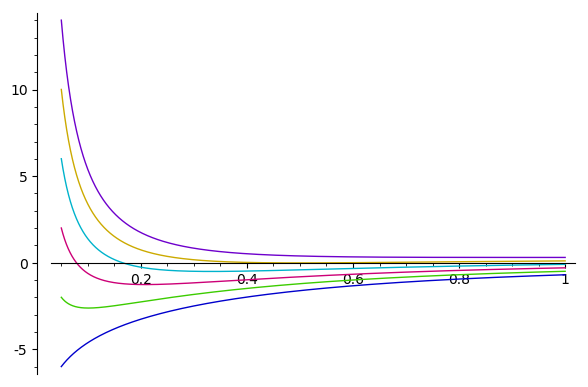
\includegraphics[width=8cm]{output_5_0.png}
		\caption{Plot of $U(q)$ for $\alpha = 0, 0.2, 0,4,...,1.0$. $\alpha = 1$ yields the purple curve and for $\alpha = 0$ we obtain the blue curve.}
	\end{figure}

	

	\item 
	\begin{figure}[H]
		\centering
		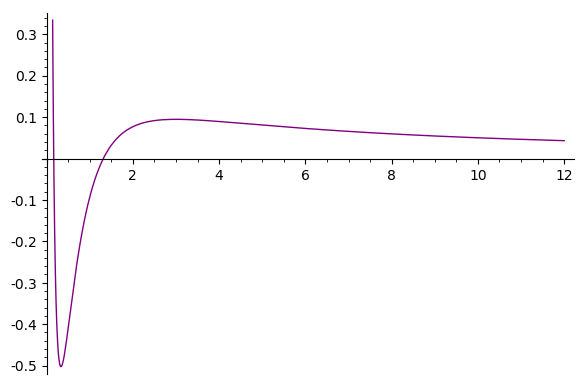
\includegraphics[width=8cm]{output_6_0.png}
		\caption{Plot of $U(q)$ for $\alpha = 0.6$.}
	\end{figure}
	Consider the graph of $U(q)$ with parameter $\alpha = 0.6$. We will discuss the behaviour of this particular dynamical system, however it applies for every dynamical system with $0<\alpha < 1$ since all these systems have the same kind of critical points. For $\alpha \geq 1$ there are no critical points, i.e. the system just escapes to the right and potential energy decreases while the kinetic energy becomes larger until the kinetic energy is equal to the total energy. We will also see that for $0 < \alpha < 1$ there exists closed orbits, i.e. periodic orbits.

	First, assume the total energy of the system is $E_0$. That means, when a particle starts at $x_0$ the potential energy is $E_0$ and the kinetic energy is zero. If the particle is at any position $x > x_0$ with velocity $\dot x < 0$, the particle moves to the left until it reaches $x_0$ for the total energy is a conserved quantity and cannot exceed $E_0$. If the particle reaches $x_0$, the velocity of the particle is zero and the slope of $U$ at $x_0$ is negative and therefore the force $F(x_0)$ is positive (note that $F = -dU$). The motion of $x$ thus turns at $x_0$ and $\dot x > 0$. The particle moves to the right and escapes to infinity.
	
	Now, assume the total energy of the system is lower than $U(x_{max})$. Let $E_1$ denote the total energy for such system. If the particle is at $x > x_{max}$ the discussion is similar to that above; the particle just escapes to the right. If the particle lies between $x_1$ and $x_{2}$ it remains bounded in this intervall for all time. At $x_1$ the potential energy is highest and the force $F$ is positive. The particle is pushed to the right until it reaches $x_{2}$. There, the kinetic energy is zero and the slope of $U$ is positive. Thus, the force is negative and the particle is pushed to the left until it reaches $x_1$ again. So, the particle moves back and forth inside the interval $[x_1,x_2]$ due to $F(x_1) > 0$ and $F(x_2) < 0$. This behaviour is reflected in a close orbit of the phase portrait.
	
	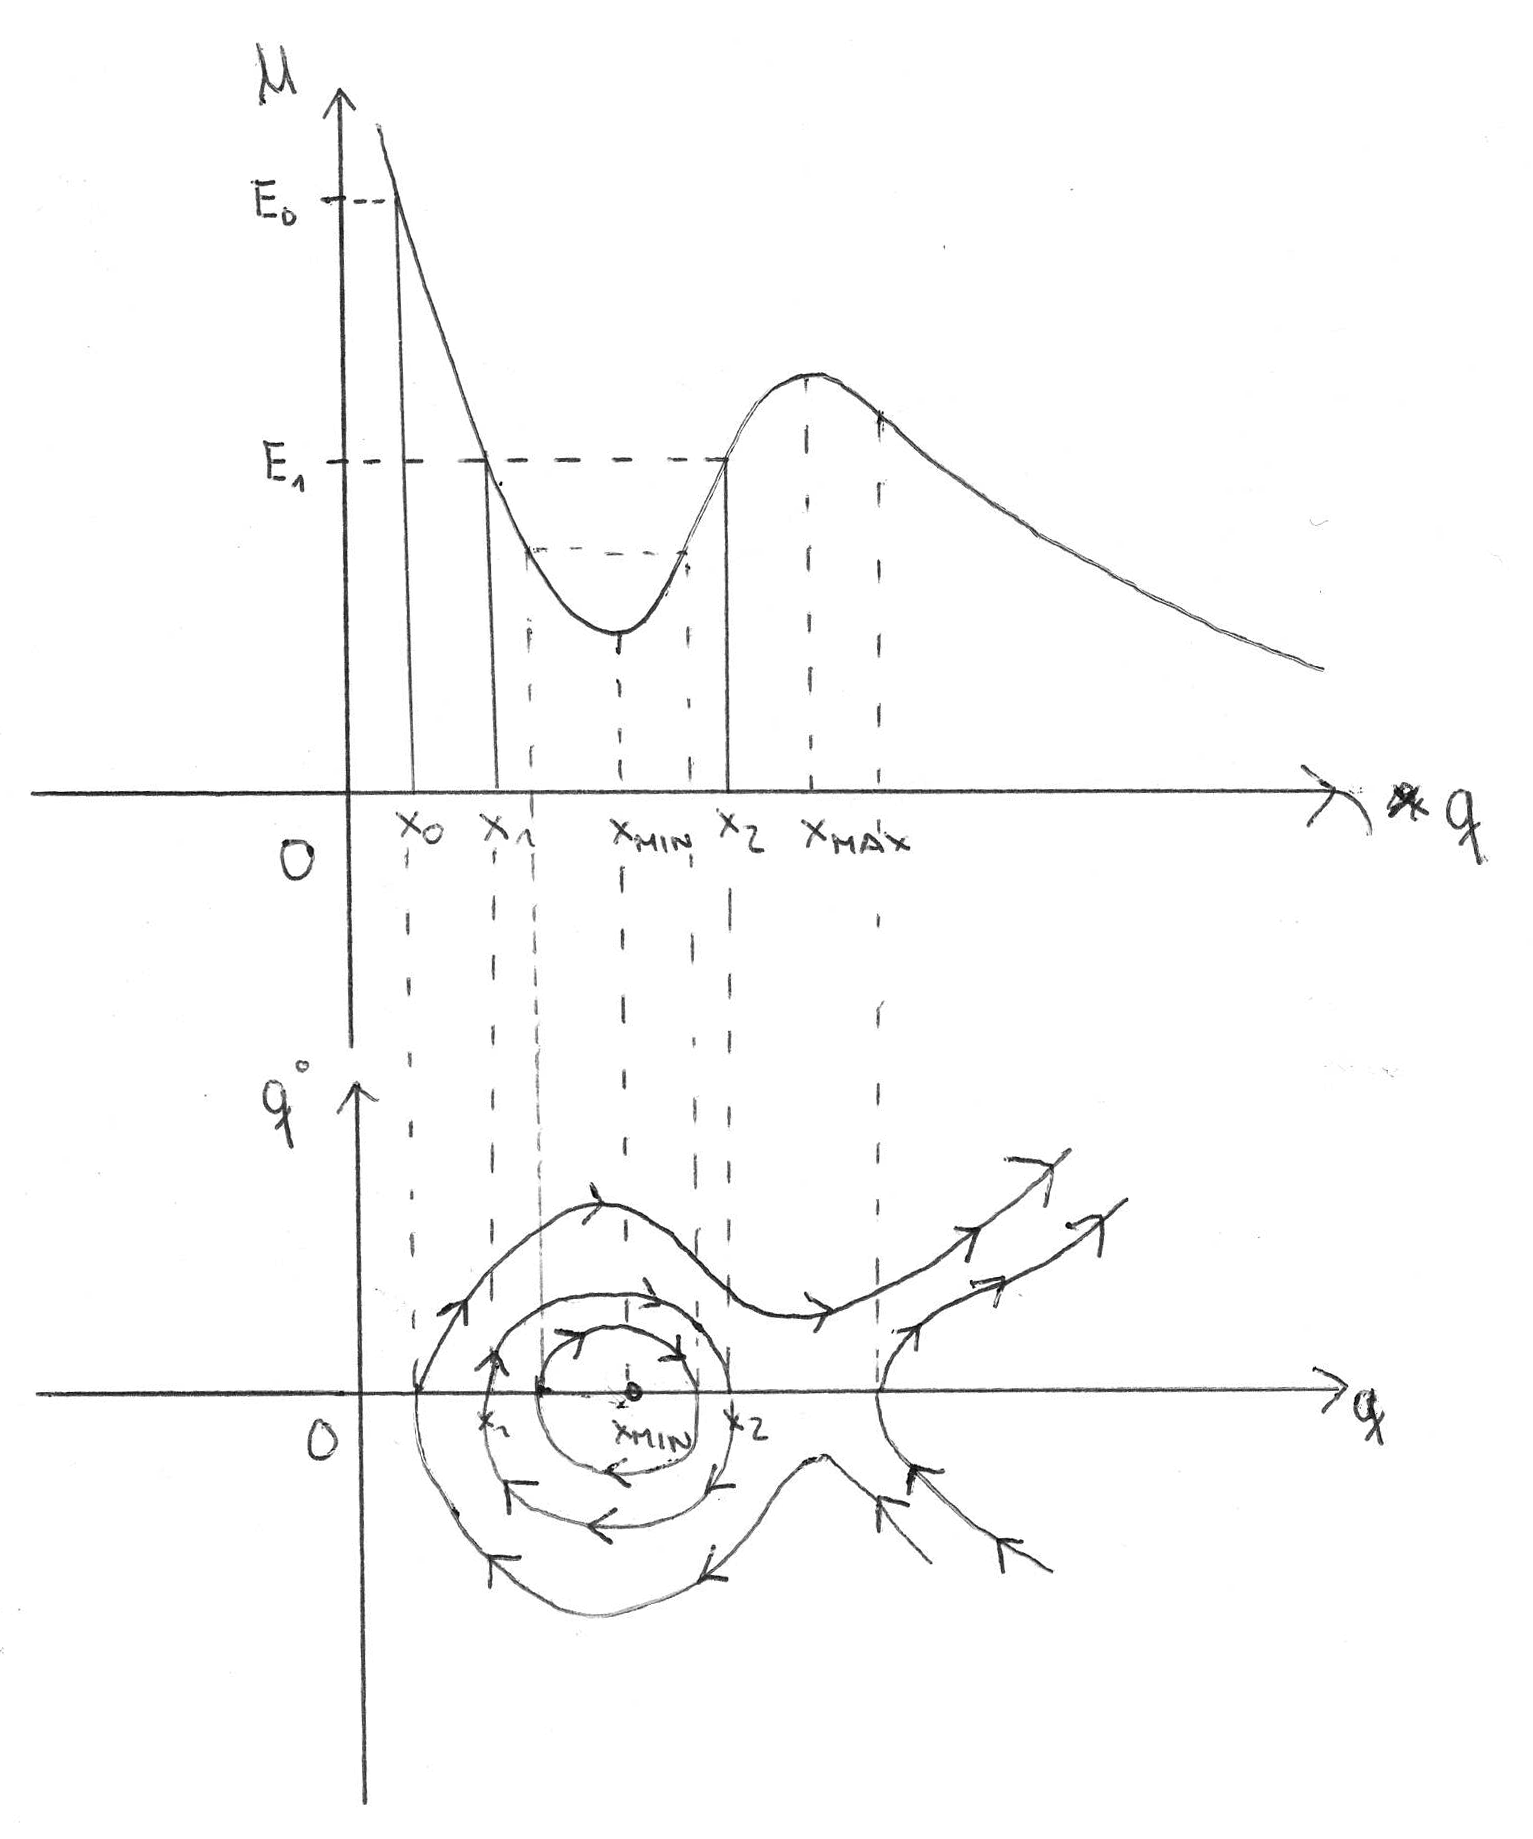
\includegraphics[width=16cm]{UE10-01-phaseportrait.png}
\end{enumerate}


\section*{Exercise 10.2}
\begin{enumerate}[label=(\alph*)]
	\item The Lagrange function is given by $\mathcal L(q, \dot q, t) = e^{\frac{\alpha}{m} t}[\frac{1}{2} m \langle \dot q, \dot q \rangle - U(q)]$. We are looking for the Euler-Lagrange equations $E\mathcal L_i = 0$ for $i = 1,...,n$, where $E \mathcal L_i = \frac{\partial \mathcal L}{\partial q_i} - \frac{d}{dt}(\frac{\partial L}{\partial \dot q_i})$. First, we compute 
	$$\frac{\partial \mathcal  L}{\partial q_i} = -e^{\frac{\alpha}{m} t} \frac{\partial U(q)}{\partial q_i}.$$
	Next, it is $$\frac{\partial \mathcal L}{\partial \dot q_i} = \frac{1}{2}me^{\frac{\alpha}{m}t} \frac{\partial}{\partial \dot q_i} \langle \dot q_i, \dot q_i \rangle =  \frac{1}{2}me^{\frac{\alpha}{m}t} \sum_{j=1}^n \frac{\partial}{\partial \dot q_i} \dot q_j^2 = \frac{1}{2}me^{\frac{\alpha}{m}t} \cdot 2 \dot q_i = m\dot q_i e^{\frac{\alpha}{m}t}.$$
	 Finally, we have 
	$$\frac{d}{dt} \frac{\partial L}{\partial \dot q_i} = \frac{d}{dt} m\dot q_i e^{\frac{\alpha}{m}t} = \alpha \dot q_i e^{\frac{\alpha}{m}t} + m\ddot q_i e^{\frac{\alpha}{m}t} = e^{\frac{\alpha}{m}t}(\alpha \dot q_i + m \ddot q_i).$$
	 So we get for $E \mathcal L_i = 0$ that
	\[
		 e^{\frac{\alpha}{m}t}(\alpha \dot q_i + m \ddot q_i) + e^{\frac{\alpha}{m} t} \frac{\partial U(q)}{\partial q_i} = 0 \iff e^{\frac{\alpha}{m}t}[\alpha \dot q_i + m \ddot q_i + \frac{\partial U(q)}{\partial q_i}]= 0 \tag{\text{Euler-Lagrange equations}}.
	\]
	
	\item Let $m = 1$ and $U(q) = -\beta q$ with $\beta > 0$. We consider the case in $\mathbb R$. The derivative of $U$ is $U'(q) = -\beta$. Hence, the Euler-Lagrangre equations reads (after division by $e^{\frac{\alpha}{m}t} \neq 0$)
	\[
		m \ddot q + \alpha \dot q = \beta.
	\]
	The characteristic polynomial is $\lambda(m \lambda + \alpha )= 0$ and has roots at $\lambda_1 = 0$ and $\lambda_2 = - \frac{\alpha}{m}$. So the homogeneous solution is
	\[
		q_{hom}(t) = c_1 + c_2 e^{-\frac{\alpha}{m}t}, \quad c_1,c_2 \in \mathbb R.
	\]
	To obtain a particular solution, we try the ansatz $q_{par}(t) = \mu t$. Substituting into the Euler-Lagrange equation gives $\alpha \mu = \beta$ and from this follows $\mu = \frac{\beta}{\alpha}$. Overall, we obtain a solution by
	\[
		q(t) = q_{hom}(t) + q_{par}(t) = c_1 + c_2 e^{-\frac{\alpha}{m}t} + \frac{\beta}{\alpha}t.
	\]
	Now, we have to consider the initial values with $q(0) = q_0 > 0$ and $\dot q(0) = 0$. The derivative of $q$ is $q'(t) = \frac{-\alpha}{m}c_2 e^{-\frac{\alpha}{m} t} + \frac{\beta}{\alpha}$. If we set $c_2 = \frac{\beta m}{\alpha^2}$, we see that it satisfies the constraint:
	$$q'(0) =  \frac{-\alpha}{m} \cdot \frac{\beta m}{\alpha^2} + \frac{\beta}{\alpha} = \frac{-\beta}{\alpha} + \frac{\beta}{\alpha} = 0.$$
	At the end, we have 
	\[
		q(0) = c_1 + \frac{\beta m}{\alpha^2} = q_0 \iff c_1 = q_0 - \frac{\beta m}{\alpha^2}.
	\]
	The curve $q(t) = q_0 - \frac{\beta m}{\alpha^2} + \frac{\beta m}{\alpha^2} e^{-\frac{\alpha}{m}t} + \frac{\beta}{\alpha}t$ solves the Euler-Lagrange equation.
	
	We calculate the behaviour of $\dot q$ for $t \to \infty$.
	\[
		\lim_{t \to \infty} \dot q(t) = \lim_{t \to \infty} -\frac{\beta}{\alpha}e^{-\frac{\alpha}{m}t} + \frac{\beta}{\alpha} = \frac{\beta}{\alpha}.
	\]
\end{enumerate}

\section*{Exercise 10.3}
\begin{enumerate}[label=(\alph*)]
	\item Compute the Euler-Lagrange equations as follows
	\begin{gather*}
		\frac{\partial \mathcal L}{\partial q_1} = \alpha \dot q_2, \quad \frac{\partial \mathcal L}{\partial q_2} =- \alpha \dot q_1, \quad \frac{\partial \mathcal L}{\partial q_3} = 0, \\
		\frac{\partial \mathcal L}{\partial \dot q_1} = \dot q_1 - \alpha q_2, \quad \frac{\partial \mathcal L}{\partial \dot q_2} = \dot q_2 + \alpha q_1, \quad \frac{\partial \mathcal L}{\partial \dot q_3} = \dot q_3 \\
		\frac{d}{dt}\frac{\partial \mathcal L}{\partial \dot q_1} = \ddot q_1 - \alpha \dot q_2, \quad 	\frac{d}{dt}\frac{\partial \mathcal L}{\partial \dot q_2} = \ddot q_2 + \alpha \dot q_1, \quad 	\frac{d}{dt}\frac{\partial \mathcal L}{\partial \dot q_3} = \ddot q_3
	\end{gather*}
	We obtain
	\[
		\begin{cases}
			2\alpha \dot q_2 - \ddot q_1 = 0 \\
			2 \alpha \dot q_1 + \ddot q_2 = 0 \\
			\ddot q_3 = 0.
		\end{cases}
	\]
	
	\item The rotation around the $q_3$-axis is given by 
	\[
		\Psi_{\varphi}(q) = \begin{pmatrix}
			q_1 \cos \varphi - q_2 \sin \varphi \\
			q_1 \sin \varphi + q_2 \cos \varphi \\
			q_3
		\end{pmatrix} \text{ and } \; \frac{d}{dt}\Psi_{\varphi}(q)= \begin{pmatrix}
		\dot q_1 \cos \varphi - \dot q_2 \sin \varphi \\
		\dot q_1 \sin \varphi + \dot q_2 \cos \varphi \\
		\dot q_3
		\end{pmatrix}, \quad \varphi \in [0, 2 \pi).
	\]
	So, the Euler-Lagrange function with the new coordinates is
	\begin{align*}
		\mathcal L\left(	\Psi_{\varphi}(q),  \frac{d}{dt} \Psi_{\varphi}(q) \right) &=
		\frac{1}{2}\left[ (\dot q_1 \cos \varphi - \dot q_2 \sin \varphi)^2 + (\dot q_1 \sin \varphi + \dot q_2 \cos \varphi)^2 + \dot q_3^2 \right] \\
		&\quad +\alpha [ 
			(q_1\cos\varphi - q_2 \sin\varphi)(\dot q_1 \sin \varphi - \dot q_2 \cos \varphi)	 - ( q_1 \sin \varphi + q_2 \cos \varphi)(\dot q_1 \cos \varphi - \dot q_2 \sin \varphi)	
		] \\
		&\Downarrow \text{SageMath simplifies the second bracket to} \\
		&= \frac{1}{2}\left[ (\dot q_1 \cos \varphi - \dot q_2 \sin \varphi)^2 + (\dot q_1 \sin \varphi + \dot q_2 \cos \varphi)^2 + \dot q_3 \right] 
		 + \alpha[
			-q_2 \dot q_1 + q_1 \dot q_2
		] \\
		&\Downarrow \text{SageMath simplifies this to} \\
		&= -\alpha q_2 \dot q_1 + \alpha q_1 \dot q_2 + \frac{1}{2}(\dot q_1^2 + \dot q_2^2 + \dot q_3^2).
	\end{align*}
	We easily see that
	\begin{gather*}
		\frac{\partial \mathcal L}{\partial q_1} = \alpha \dot q_2, \quad \frac{\partial \mathcal L}{\partial q_2} =- \alpha \dot q_1, \quad \frac{\partial \mathcal L}{\partial q_3} = 0, \\
		\frac{\partial \mathcal L}{\partial \dot q_1} = \dot q_1 - \alpha q_2, \quad \frac{\partial \mathcal L}{\partial \dot q_2} = \dot q_2 + \alpha q_1, \quad \frac{\partial \mathcal L}{\partial \dot q_3} = \dot q_3 \\
		\frac{d}{dt}\frac{\partial \mathcal L}{\partial \dot q_1} = \ddot q_1 - \alpha \dot q_2, \quad 	\frac{d}{dt}\frac{\partial \mathcal L}{\partial \dot q_2} = \ddot q_2 + \alpha \dot q_1, \quad 	\frac{d}{dt}\frac{\partial \mathcal L}{\partial \dot q_3} = \ddot q_3
	\end{gather*}
	Compare it with the solution at the beginning, and we see that the system is invariant under rotation.
	
\end{enumerate}

\end{document}
